% Section 3: Threats and Promises
%-------------------------------------------------------------------------------

\begin{frame}{Examples of Threats and Promises}
  \begin{center}
    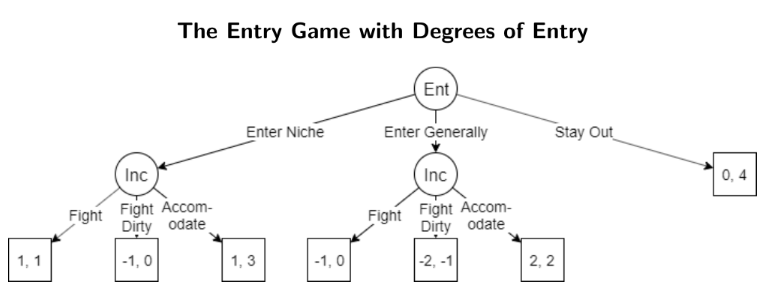
\includegraphics[width=1\textwidth]{figures/entrygame.png} 
  \end{center} 
  What is the \textbf{SPNE}?
\end{frame}

% - - - - - - - - - - - - - - - - - - - - - - - - - - - - - - - - - - - - - - - 

\begin{frame}{Examples of Threats and Promises}
  \begin{center}
    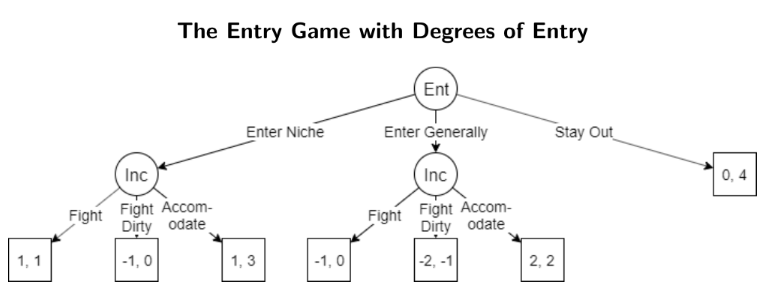
\includegraphics[width=.7\textwidth] {figures/entrygame.png}
  \end{center} 
  Examples of threats/promises that \alert{Incumbent} could make:
  \begin{itemize}
    \item ``If you enter niche, I will Fight; If you enter generally, I will Fight Dirty''
    \item ``If you enter niche, I will Accommodate; If you enter generally, I will Fight''
    \item ``If you enter niche \textit{or} generally, I will Fight Dirty''
  \end{itemize}
\end{frame}

% - - - - - - - - - - - - - - - - - - - - - - - - - - - - - - - - - - - - - - - 

\begin{frame}{Examples of Threats and Promises}
  \begin{center}
    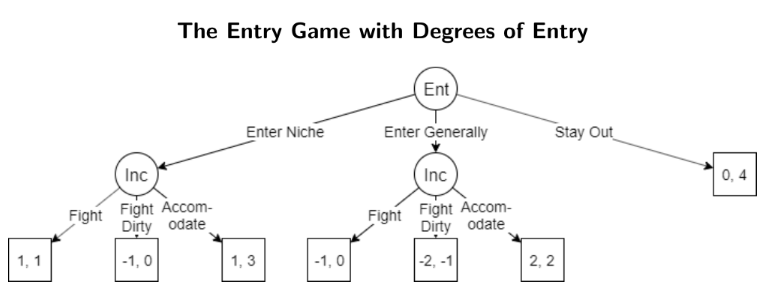
\includegraphics[width=.7\textwidth] {figures/entrygame.png}
  \end{center} 
  What is the \textbf{optimal commitment} for the \alert{Incumbent} to make? \\
  How can they be made credible?
\end{frame}

% - - - - - - - - - - - - - - - - - - - - - - - - - - - - - - - - - - - - - - - 

\begin{frame}{Examples of Threats and Promises}
  \begin{center}
    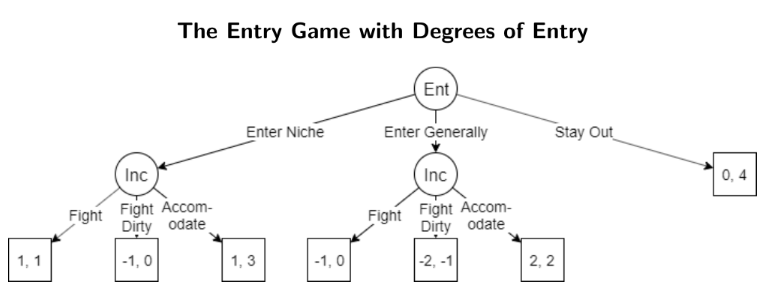
\includegraphics[width=.7\textwidth] {figures/entrygame.png}
  \end{center} 
  {Stay Out, (Fight Dirty, Fight)} \textit{is} a NE of this game, just not \textit{subgame-perfect}
  \begin{itemize}
    \item An interpretation for those non-subgame-perfect NEs is that they exist as the result of such threats 
  \end{itemize}
\end{frame}

% - - - - - - - - - - - - - - - - - - - - - - - - - - - - - - - - - - - - - - - 

\begin{frame}{Examples of Threats and Promises}
  \begin{center}
    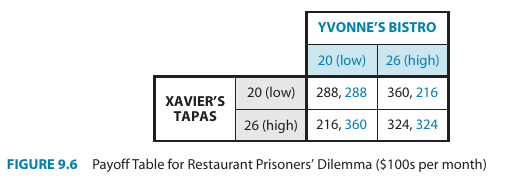
\includegraphics[width=.8\textwidth]{figures/fig96.png} 
  \end{center} 
  Consider the promise ``I will charge a high price if you do'' \\
  Sounds good right?
\end{frame}

% - - - - - - - - - - - - - - - - - - - - - - - - - - - - - - - - - - - - - - - 

\begin{frame}{Examples of Threats and Promises}
  \begin{center}
    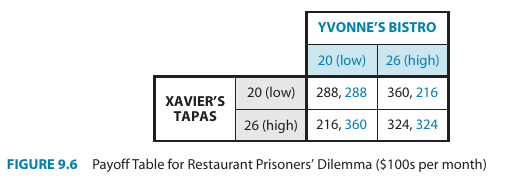
\includegraphics[width=.6\textwidth]{figures/fig96.png} 
  \end{center}
  What if Xavier \textit{promises} to set a high price?
  \begin{itemize}
    \item Should Yvonne believe him? 
    \item How can Xavier \textit{credibly commit} to not undercutting Yvonne when he sees she has set a high price?
    \begin{itemize}
      \item Handing off the decision to a trusted 3rd party (commitment),
      \item Develop a reputation of honesty (change his payoffs)
    \end{itemize}
  \end{itemize}
\end{frame}

% - - - - - - - - - - - - - - - - - - - - - - - - - - - - - - - - - - - - - - - 

\begin{frame}{Deterrence of Entry (Harrington)}
  \begin{center}
    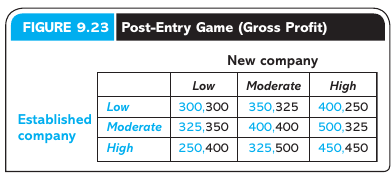
\includegraphics[width=.6\textwidth]{figures/fig923.png} 
  \end{center}
  Consider a market with an established and a potential new entrant:
  \vspace{-5mm}
  \begin{itemize}
    \item Established monopolist would usually earn 1,000 profit 
    \item If competing, each company could set \textit{low}, \textit{moderate}, \textit{high} price
    \item Start-up cost to entrant is 350.
  \end{itemize}
\end{frame}

% - - - - - - - - - - - - - - - - - - - - - - - - - - - - - - - - - - - - - - - 

\begin{frame}{Deterrence of Entry}
  \begin{center}
    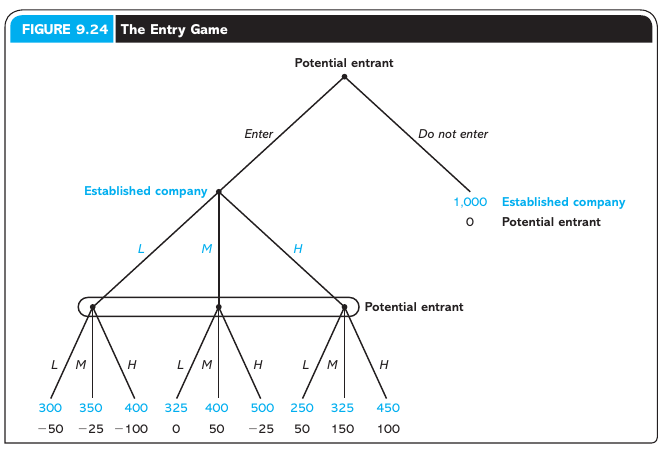
\includegraphics[width=.9\textwidth]{figures/fig924.png}
  \end{center} 
  What is the \textbf{SPNE}?
\end{frame}

% - - - - - - - - - - - - - - - - - - - - - - - - - - - - - - - - - - - - - - - 

\begin{frame}{Deterrence of Entry}
  \begin{center}
    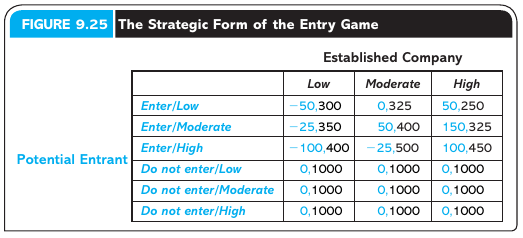
\includegraphics[width=.9\textwidth]{figures/fig925.png}
  \end{center} 
  Can you find NE which are \textit{not subgame-perfect}?
\end{frame}

% - - - - - - - - - - - - - - - - - - - - - - - - - - - - - - - - - - - - - - - 

\begin{frame}{Deterrence of Entry}
  Consider \{Do not enter/Moderate, Low\}:
  \begin{itemize}
    \item Given no entry, established company always gets 1,000
    \item So planning to set a low price in post-entry game is optimal for est. company
    \item Given that est. company prices low, new company has no regrets staying out 
    \item If new company enters when est. company sets low price, the best they can do is \textit{moderate} and earn -25
  \end{itemize}
\end{frame}

% - - - - - - - - - - - - - - - - - - - - - - - - - - - - - - - - - - - - - - - 

\begin{frame}{Deterrence of Entry}
  Consider \{Do not enter/Moderate, Low\}:
  \begin{itemize}
    \item Why is this \textit{not} subgame-perfect?
    \item Consider what happens if the new company doesn't believe the threat, 
    and actually \textit{does} enter
    \item Then the established firm would actually be better off by setting a \textit{moderate} price
    \item So we say that the threat of low price competition was not a \textbf{credible} threat
  \end{itemize}
\end{frame}

\begin{frame}{Deterrence of Entry}
  So what should the CEO of an established company do? 
  \begin{itemize}
    \item How can they commit to an aggressive pricing strategy that they know they won't follow through on? 
    \item What if there is a \textit{costly} investment in a new technology which has an investment cost of 500,
    but lowers per-unit production costs
  \end{itemize}
\end{frame}

\begin{frame}{Deterrence of Entry}
  \begin{center}
    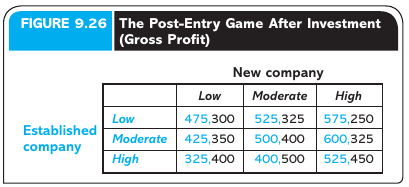
\includegraphics[width=.8\textwidth]{figures/fig926.png}
  \end{center} 
  What is the NE of this new post-entry game?
\end{frame}

\begin{frame}{Deterrence of Entry}
  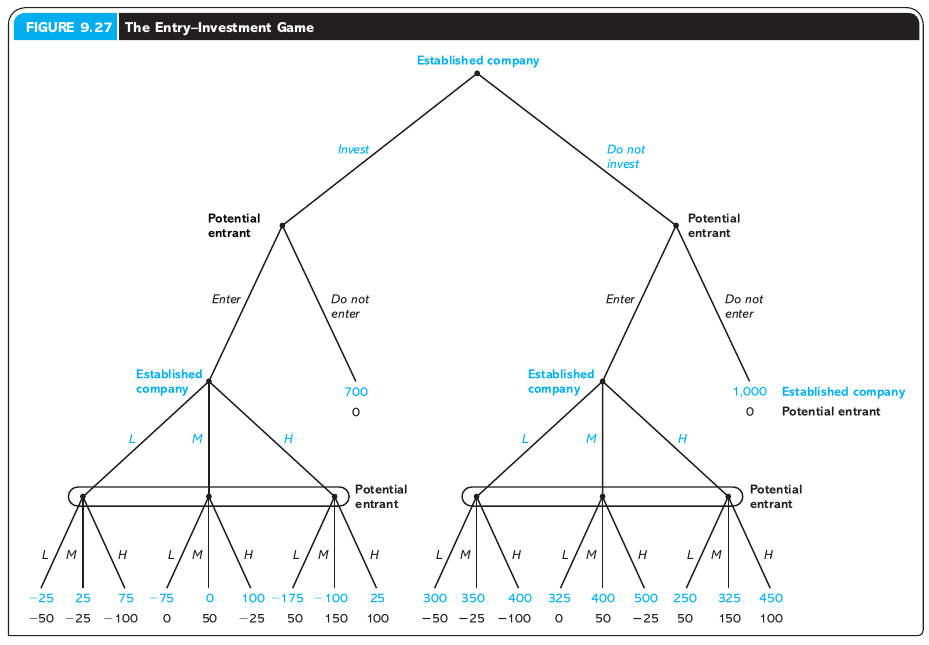
\includegraphics[width=1\textwidth]{figures/fig927.png} 
\end{frame}

\begin{frame}{Deterrence of Entry}
  \begin{center}
  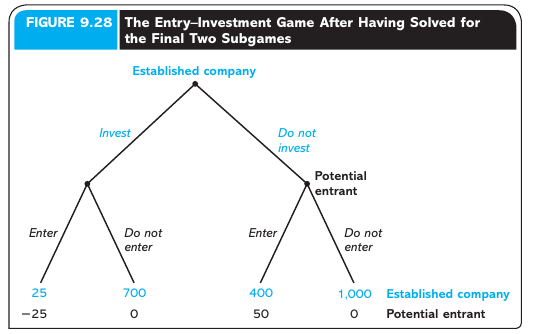
\includegraphics[width=.8\textwidth]{figures/fig928.png}
  \end{center}
  What is the \textbf{SPNE} now?
  \begin{itemize}
    \item Is the aggressive pricing strategy \textit{credible} now? 
  \end{itemize}
\end{frame}

\begin{frame}{Deterrence of Entry}
  \begin{center}
    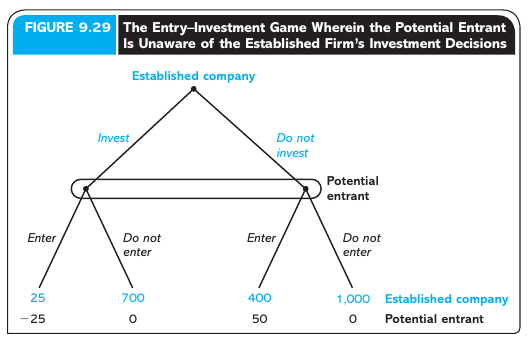
\includegraphics[width=.7\textwidth]{figures/fig929.png} 
  \end{center}
  Consider the importance of communicating the investment
  \begin{itemize}
    \item What is the SPNE when the potential entrant can't see whether the established company has invested? 
  \end{itemize}
\end{frame}

\begin{frame}{A Doomsday Device}
  Spoilers for \textit{Doctor Strangelove or: How I Learned to Stop Worrying and Love the Bomb} (1964)
  \begin{quote}
    \footnotesize
    \textbf{Dr. Strangelove:} Mr. President, it is not only possible, it is essential. That is the whole idea of this machine, you know. Deterrence is the art of producing in the mind of the enemy . . . the fear to attack. And so, because of the automated and irrevocable decision making process which rules out human meddling, the doomsday machine is terrifying. It’s simple to understand. And completely credible, and convincing. (Turning to DeSadeski.) But the whole point of the doomsday machine is lost if you keep it a secret! Why didn’t you tell the world, eh?

    \textbf{Soviet Ambassador DeSadeski:} It was to be announced at the Party Congress on Monday. As you know, the Premier loves surprises.
  \end{quote}
\end{frame}
